\documentclass[../primer.tex]{subfiles}

\begin{document}

%% --------------------------------------------------
\chapter{Wrangle} \label{ch:wrangle}
%% --------------------------------------------------
After clearly formulating our question(s), finding and exploring the available
data, obtaining and assessing a relevant model, we may proceed to
\textbf{wrangling} the uncertainty.

If we are pursuing a predictive simulation, we might carry out \textbf{forward
  propagation} -- compute the uncertainty in $Y$ based on the input uncertainty
in $\mX$. We might use the same techniques to support model validation.

If we are attempting to determine some un-measurable physical quantity with the
aid of a model and physical data, we might carry out \textbf{inverse
  propagation}, also called inference.

The forward and reverse problems are rather different in character, but both
are affected by the \textbf{curse of dimensionality}.

\section{Dimensionality}
%% --------------------------------------------------
The \textbf{curse of
  dimensionality}\footnote{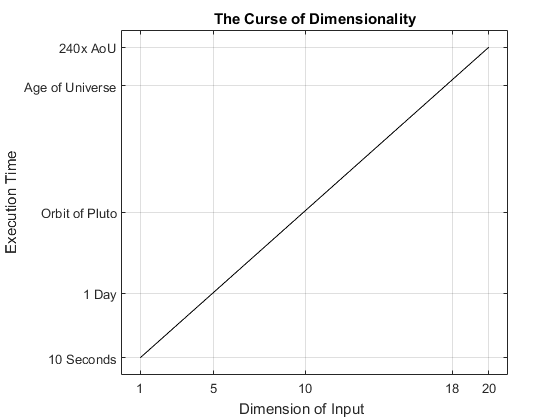
\includegraphics[width=0.50\textwidth]{./images/curse_of_dimensionality}\\ Recall
  that na\"ive execution time scales \emph{exponentially} with the number of
  dimensions.} manifests in many ways,

\section{Forward}
%% --------------------------------------------------
\textbf{Forward propagation} of uncertainty maps uncertainty from the inputs
$\mX$ to uncertainty in the output $Y$. Conceptually this is simple -- we map
via the function $Y = f(\mX)$. Computationally this can be challenging: High
dimensionality explodes the cost, and expensive simulators for $f$ exacerbate
the issue. We will consider a few strategies for tackling forward propagation.

\subsection{Delta Method}
%% --------------------------------------------------
The \textbf{delta method} is essentially a Taylor approximation, analyzed for
distributional assumptions. The high-level observation is that if parameters
$\v\theta$ are estimated from data, then the estimate $\hat{\v\theta}$ ought to
grow closer to the true value $\v\theta$ as the number of samples $m$ is
increased. As this distance is reduced, a Taylor approximation will be
increasingly accurate.

For instance,\cite{van1998asymptotic} if we have an estimator that satisfies

\begin{equation} \label{eq:ch4-delta-est}
  \hat{\v\theta} \stackrel{d}{\to} \dN(\v\theta, \m\Sigma^2/n),
\end{equation}

\noindent with $\m\Sigma\in\R{d\times d}$ a covariance matrix,\footnote{note
  that $\stackrel{d}{\to}$ denotes \emph{convergence in distribution}, a
  particular form of convergence for random variables} then we have

\begin{equation} \label{eq:ch4-delta-fcn}
  F(\hat{\v\theta}) \stackrel{d}{\to} %
  \dN\left(F(\v\theta),
    \left.\nabla_{\v\theta}F\right|_{\v\theta}^{\top}\left(\m\Sigma^2/n\right) %
      \left.\nabla_{\v\theta}F\right|_{\v\theta}\right).
\end{equation}

\noindent \Cref{eq:ch4-delta-fcn} provides an \emph{asymptotic} distribution --
an approximation that grows increasingly accurate with increased $n$. Note also
that this approximation depends on unknown quantities $\v\theta,\m\Sigma$; we
may introduce an additional level of approximation by using estimates
$\hat{\v\theta},\hat{\m\Sigma}$. In practice we may need to approximate the
gradient of $f$ at $\hat{\v\theta}$; this grows only linearly in dimension.

Finally, notice that we have switched notation for this example, and are
considering functions of parameters $F(\v\theta)$, rather than random variables
$f(\mX)$. The delta method only makes sense as an approximation when it is
reasonable to assume \emph{there exists a true value} $\v\theta$. If we are
interested in a function of a random variable $\mX$, we will have to turn to a
different approach.\footnote{The delta method can still be useful \emph{in
    conjunction} with other methods introduced below. We will consider
  techniques to approximate expectations $F(\v\theta) = \E[f(\mX)|\v\theta]$
  conditional on particular parameter values. If the particular values are not
  known, but instead estimated $\hat{\v\theta}$, we have a propagation task
  appropriate for the delta method. In this case, we might use the likelihood
  ratio method for approximating the gradient.\cite{l1990unified}}

\subsection{Monte Carlo}
%% --------------------------------------------------
The Monte Carlo method is a simple, flexible means to propagate uncertainty. If
we have a distribution for our random variables $\mX\sim\rho$, Monte Carlo
simply involves drawing independent samples $\mX_i\sim\rho$ for $i=1,\dots,m$,
and evaluating those samples $Y_i = f(\mX_i)$ to construct an empirical
distribution for the output.

We often use Monte Carlo to approximate an expectation;\footnote{Remember from
  probability theory that many useful quantities can be expressed as
  expectations; for instance, a probability of exceeding some threshold $\P[Y>y]
  = \E[H(Y-y)]$, where $H(\cdot)$ is the Heaviside function. We can think of
  this as modifying the function that maps the inputs $\mX$; in the previous
  example the new function is $H(f(\mX)-y)$.} the Monte Carlo estimate for the
mean of $Y$ is given by

\begin{equation} \label{eq:ch4-mc-mean}
  \hat{\mu}_m = \frac{1}{m}\sum_{i=1}^m Y_i.
\end{equation}

\noindent \Cref{eq:ch4-mc-mean} is called a Monte Carlo estimate for $\E[Y]$ --
it is a sample mean, as discussed above in Section \ref{sec:ch3-data}. The law
of large numbers guarantees that as $m\to\infty$, the Monte Carlo estimate
approaches its true value -- so long as the true value
exists.\cite{owen2013montecarlo}\footnote{That is, the target expectation must
  be finite.}

Note that we have taken a \emph{deterministic} quantity $\E[Y]$, and constructed
a \emph{random variable estimate} $\hat{\mu}_m$. The Monte Carlo estimate has
variance equal to

\begin{equation} \label{eq:ch4-mc-var}
  \E[(\hat{\mu}_m - \E[Y])^2] = \frac{\V[Y]}{m},
\end{equation}

\noindent so long as $\V[Y]$ is finite. The standard error $\sqrt{\V[Y]/m}$ is
the relevant notion of accuracy for this estimation method. \Cref{eq:ch4-mc-var}
implies that \emph{Monte Carlo is slow to converge} -- the standard error
decreases as $1/\sqrt{m}$, which is rather inefficient compared to other
techniques. On the other hand, the standard error depends only on the true
variance of $Y$ and the number of samples $m$ -- \emph{it is independent of
  dimension $d$}.\footnote{So long as $\V[Y]$ does not grow with $d$.} This is
an important observation: In very high-dimensional settings, Monte Carlo is our
only viable option for propagation.

The particular approach described above is called \emph{simple} Monte Carlo;
there exist many different formulations of Monte Carlo that seek to improve
convergence or handle particular issues. For instance, in some cases it is not
possible to draw samples from the given distribution $\rho$, particularly when
the target distribution is not known in closed form. In this case, a flavor of
Monte Carlo might be used just to generate samples $\mX_i$. For more on Monte
Carlo, a good introduction is Reference \cite{owen2013montecarlo}.

\subsection{Quadrature}
%% --------------------------------------------------
An alternative

\section{Inverse} \label{sec:inverse-propagation}
%% --------------------------------------------------

\subsection{Sanity checks}
% -------------------------
\textcolor{red}{TODO} Inference for sanity checks; falling box inferring g example

\end{document}
